\documentclass{article}
\usepackage[utf8]{inputenc}
\usepackage[a4paper, margin=2.5cm]{geometry}
\usepackage{graphicx}
\usepackage[french]{babel}

\usepackage[default,scale=0.95]{opensans}
\usepackage[T1]{fontenc}
\usepackage{amssymb} %math
\usepackage{amsmath}
\usepackage{amsthm}
\usepackage{systeme}
\usepackage{cases}

\usepackage{hyperref}
\hypersetup{
    colorlinks=true,
    linkcolor=blue,
    filecolor=magenta,      
    urlcolor=cyan,
    pdftitle={Overleaf Example},
    % pdfpagemode=FullScreen,
    }
\urlstyle{same} %\href{url}{Text}

\theoremstyle{plain}% default
\newtheorem{thm}{Théorème}[section]
\newtheorem{lem}[thm]{Lemme}
\newtheorem{prop}[thm]{Proposition}
\newtheorem*{cor}{Corollaire}
%\newtheorem*{KL}{Klein’s Lemma}

\theoremstyle{definition}
\newtheorem{defn}{Définition}[section]
\newtheorem{exmp}{Exemple}[section]
% \newtheorem{xca}[exmp]{Exercise}

\theoremstyle{remark}
\newtheorem*{rem}{Remarque}
\newtheorem*{note}{Note}
%\newtheorem{case}{Case}



\title{Cours}
\author{Charles Vin}
\date{Date}

\begin{document}
\maketitle

\underline{Nouveau cours de la rentrée} \\
... \\ 
\underline{Nouveau cours du 17/01} \\

\textbf{Rappel}:

\begin{align*}
    (P) &\min f(x) \\
    S.C &\systeme*{
        g(x) = 0
        h(x) \leq 0
        x \in \Omega 
    }
    \mathcal{A} = \{x \in \Omega : g(x) = 0, h(x) \leq 0\}
\end{align*}

\textbf{Convexité}
\begin{itemize}
    \item Un ensemble E est un convexe si 
    \[
        \forall x,y \in E, \forall t \in {0,1} tx + (1-t)y \in E
    .\]
    \item Soit $ f $ une fonction de $ \mathbb{R}^n $ dans $ \mathbb{R} $ défini sur un convexe $ E $. Alors $ f $ est une fonction convexe si 
    \[
        \forall x,y \in E, \forall t \in [0,1] : f(tx + (1-t)y) \leq tf(x) + (1-t)f(y)
    .\]
\end{itemize}

\subsection{Problème convexes}
$ (P) $ est un problème convexe si $ f $  est une fonction convexe et $ \mathcal{A} $ est un convexe. 

En plus si $ f $ est une fonction strictement convexe alors $ (P) $ est un problème strictement convexe.

\begin{thm}[]
    Si $ (P) $ est un problème convexe et si $ x^*, (\lambda ^*, mu^*) $ vérifient les conditions KKT, alors $ X^* $ est solution optimale de $ (P) $.
\end{thm}
\begin{thm}[]
    Tout minimum locale de $ (P) $ est également minimum globales de $ (P) $. En plus l'ensemble des minimums globales est un convexe.
\end{thm}
\begin{thm}[]
    Si $ (P) $ est un problème strictement convexe et $ (P) $ admet une solution optimale, alors cette solution optimale est unique.
\end{thm}

\section{Programmation linéaire}
problème linéaire (peut s'écrire avec des matrices)
\begin{align*}
    (P) &\min C^T x \text{ (ou bien } <c,x>)\\
    S.C &\systeme*{
        Ax=b,
        Cx \leq d,
        x \in \Omega 
    }
\end{align*}

\begin{exmp}[exemple 2.1.1.2]
    \begin{align*}
        (P) & \min c_1 x_1 + c_2 x_2\\
        S.C & \systeme*{
            x_{1} + 3 x_{2} \leq 18,
            x_{1} + x_{2} \leq 8,
            2x_{1} + x_{2} \leq 14,
            x_{1} \geq 0,
            x_{2} \geq 0
        }
    \end{align*}

    \textbf{Résolution graphique}
    $ c_1 = 3, c_2 = 8 $ traduire les contraintes en droite, les dessiner trouver la zone admissible. \\
    On défini les courbes de niveau. 
    \begin{align*}
        C_k &= \{x \in \mathcal{A} : f(x)=k\} \\
            &= \{x_1,x_2 \in \mathcal{A}: 3x_1 + 8x_2 = k\}
    \end{align*}
    On a fait un truc avec ces courbe de niveau pour dire que c'était croissant puis on a choisis de prendre l'intersection de deux des équations 
    \[
        \systeme*{
            x_1 + x_2 = 8,
            x_1 + 3x_2 = 18
        } \Leftrightarrow
        \systeme*{
            2 x_2 = 10 ((II) - (I)),
            2x_1 = 6 (3(I) - (II))
        }\Leftrightarrow
        \systeme*{
            x_1 = 3,
            x_2 = 5
        } \text{ solution optimale}
    .\]
    Valeur optimale : $ 9 + 40 = 49 $ 
\end{exmp}

\begin{exmp}[]
    \begin{align*}
        c_1 = c_2 = 3 \\
        \systeme*{
            x_1 + x_2 = 8,
            X_1 + 3x_2 \leq 18,
            2x_1 + x_2 \leq 14
        } \Leftrightarrow \systeme*{
            x_2 = 8 - x_1,
            x_2 = \frac{18 - x_1}{3},
            x_2 \leq 14 - 2x_1
        } \\
        C_k = \{x_1,x_2 \in \mathbb{R} : 3x_1 + 3 x_2 = k\}\\
        \text{ étape que j'ai pas compris lol + un dessin au tableau} \\
        \text{Solution optimales } S = \{(x_1, 8-x_1 : 3 \leq x_1 \leq 6)\} = \{(8-x_2, x_2) : 2 \leq X_2 \leq 5\}
    \end{align*}
\end{exmp}

\begin{exmp}[numéros 3]
    \begin{align*}
        &\min 20x_1 + 25x_2 \\
        &\systeme*{
            x_1 + 5 x_2 \geq 5, 
            X_1 + 2x_2 \geq 4,
            3x_1 + 3x_2 \geq 6,
            x_1 \geq 0, 
            x_2 \geq 0
        } \\
        &C_k = \{x_1,x_2 \in \mathbb{R} : 3x_1 + 3 x_2 = k \} \Leftrightarrow C_100 = \{20 x_1 + 25x_2 = 100\} = \{\text{la courbe entre (0,4) et (5,0)}\} \\
        &\text{On dessine cette courbe} \\
        &\text{La fonction à min est décroissante car ...} \\
        &\text{Donc on suis les courbes parallèle à celle de Ck jusqu'a arriver au minimum} \\
        &\text{Solution optimales } \systeme*{x_1 = 0, x_2 = 2}, \text{Valeur Optimale} = 50
    \end{align*}
    \begin{figure}[!htbp]
        \centering
        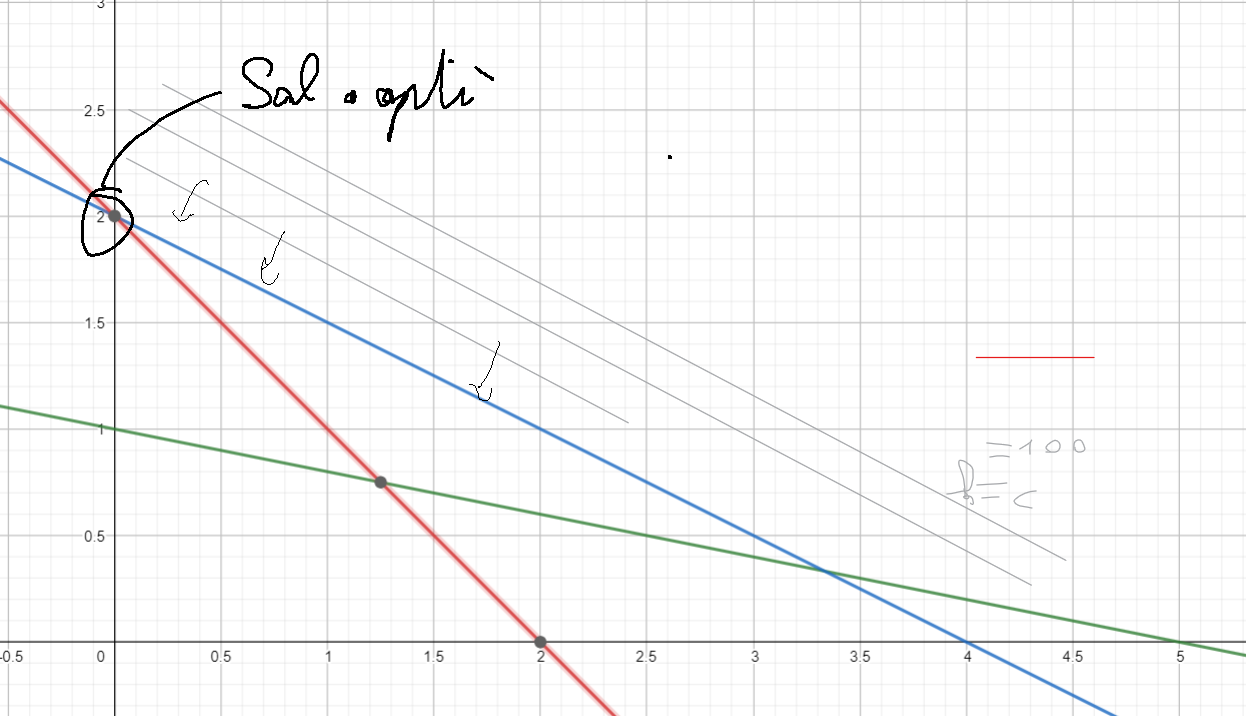
\includegraphics[width=.75\textwidth]{fig1.png}
    \end{figure}
\end{exmp}

\begin{defn}[]
    \begin{enumerate}
        \item Un polyèdre est une intersection de demiplans 
        \[
            H(a_k, b_k) = \{x \in \mathbb{R}^n, a_k x \leq  b_k\}
        .\]
        \item Un simplexe est un polyèdre borné 
        \item Un sommet est un point du polyèdre qu'on 
    \end{enumerate}
\end{defn}

\underline{Nouveau cours du 24/01} \\
\textbf{Rappel:}
\begin{enumerate}
    \item Une contraintes $ h(x) \leq 0 $ est saturée (ou <<active>>) au point $ x^* \in \mathcal{A} $ si $ h(x^*) = 0 $. \\
    Remarque : les contraintes d'égalitées $ g(x) = 0 $ sont saturées en tout $ x \in \mathcal{A} $
    \item Une matrice est de rang $ r $ si il existe une sous-matrice carrée de taille $ r $ dont le déterminant est non-null et pour toute sous-matrice de tailel plus élever le déterminant vaut 0. 
\end{enumerate}

\begin{thm}[4, p13]
    Un point $ x $ est un sommet du polyèdre $ \mathcal{A} $ si la matrice de contraintes saturées est de rang $ n $.

    Si le nombre de contraintes saturées vaut exactement $ n $ alors $ x $ est un sommet non-dégénéré. En revanche, si le nombre de contraintes saturées est strictement supérieur à $ n $, alors $ x $ est un sommet dégénéré.

    Supposons qu'on a $ p $ contraintes d'égalité, $ q $ contraintes d'inégalités, $ n $ variables. Alors le nombre de sommets du polyèdre est limité à $ \binom{q}{n-p} = \frac{q!}{(n-p)!(q-n-p)!} $ 
\end{thm}

\begin{exmp}[Exercice 12, p28]
    \begin{align*}
        (p) \systeme*{
            x_1 + 2 x_2 + 3x_3 \leq 11,
            -x_1 - 2 x_3 \leq -1,
            x_1 \leq 2,
            x_3 \leq 3,
            -x_1 \leq 0,
            -x_2 \leq 0,
            -x_3 \leq 0
        }, p)0, q=7, n=3
    \end{align*}
    Le nombre de sommets est limité par $ \binom{7}{3} = \frac{7!}{3!4!} = \frac{7*6*5}{1*2*3} = 35 $ 
    \begin{align*}
        &A = \begin{pmatrix}
            1 & 2 & 3 \\
            -1 & 0 & -2 \\
            1 & 0 & 0 \\
            0 & 0 & 1 \\
            -1 & 0 & 0 \\
            0 & -1 & 0 \\
            0 & 0 & -1
        \end{pmatrix}
        &P_1(2,0,0), \systeme*{
            2 < 11,
            -2 < -1,
            2 = 2,
            0 < 3,
            -2 < 0,
            0=0,
            0=0
        }
    \end{align*}
    
    \[
        m=3=n, A_S = \begin{pmatrix}
            1,0,0 \\
            0,-1,0 \\
            0,0,-1 \\
        \end{pmatrix}
        \det A_S = 1 \neq 0 \text{ donc } rang(A_S) = 3
    .\]
    On en déduit que $ P_1 $ est un sommet non-dégénéré.

    Autre Point : $ P_2(2,0,3) $ 
    \begin{align*}
        &P_1(2,0,0), \systeme*{
            11 = 11,
            -8 < -1,
            2 = 2,
            3 = 3,
            -2 < 0,
            0=0,
            -3 \leq 0
        }
    \end{align*}
    Les contraintes saturées sont là ou les trucs sont égales !! On remet ces équations dans la matrice $ A_S $. 
    \[
        A_S = \begin{pmatrix}
            1 & 2 & 3 \\
            1 & 0 & 0 \\
            0 & 0 & 1 \\
            0 & -1 & 0
        \end{pmatrix}
        , \det (\begin{pmatrix}
            1 & 0 & 0 \\
            0 & 0 & 1 \\
            0 & -1 & 0
        \end{pmatrix}
        ) = 1 \neq 0 \text{ donc } Rang(A_S) = 3 (=n)
    .\]
    Donc matrice dégénéré (car y'a un truc avec $ 3 = n < m $ ).

    Autre Point : $ P_3(0,5,3) $ 
    \begin{align*}
        &P_1(2,0,0), \systeme*{
            11 = 11,
            -1 = -1,
            1 < 2,
            0 < 3,
            -1 < 0,
            -5 < 0,
            0 = 0
        } m=3(=n)
    \end{align*}
    Les contraintes saturées sont là ou les trucs sont égales !! On remet ces équations dans la matrice $ A_S $. 
    \[
        A_S = \begin{pmatrix}
            1 & 2 & 3 \\
            -1 & 0 & -2 \\
            0 & 0 & -1
        \end{pmatrix}
        , \det (A_S) = -1 \det (\begin{pmatrix}1 & 2 \\ -1 & 0\end{pmatrix}) = -2 \neq 0 \text{ donc } Rang(A_S) = 3 (=n)
    .\]
    Donc $ P_3 $ est un sommet non-dégénéré
\end{exmp}

\begin{thm}[6]
    Si $ (P_L) $ admets des solutions optimales et si la matrice des contraintes est de rang $ n $, alors au moins une des solutions optimales est une sommet de $ \mathcal{A} $ 
\end{thm}

\subsection{La forme standard}
\begin{align*}
    (P_L) &\min f^Tx \\
        & s.c \systeme*{
            A_x = b,
            C x \leq d
            x \in \mathbb{R}^n
        } \\
    (P_S) &\min f^T x \\
        & s.c \systeme*{
            Ax = b,
            x \geq 0
        }
\end{align*}
Tout problème $ (P_L) $ peut s'écrire sous la forme $ (P_S) $ car
\begin{enumerate}
    \item $ \max f^T x \Leftrightarrow \min -f^Tx $ 
    \item $ a^Tx \leq b \Leftrightarrow \systeme*{a^Tx + y = b, y \geq 0} \Leftrightarrow \systeme*{a^Tx \geq b, y \geq 0} \Leftrightarrow \systeme*{a^Tx - y = b, y \geq 0}$ 
    \item $ x_k \in \mathbb{R} \Leftrightarrow
    \begin{cases} x_k = x_{k_1} - x_{k_2} \\ x_{k_1}, x_{k_2} \geq 0 \end{cases}$
\end{enumerate}

\begin{exmp}[Exercice 14 page 28]
    \begin{align*}
        (P_L) &\max x_1 + 5x_2 + 2x_3 \\ 
            & S.C \begin{cases}
                x_1 + 3x_2 \leq 10 \\
                x_1 + x_2 + x_3 \leq 9 \\
                x_1, x_3 \geq 0 \\ 
                x_2 \in \mathbb{R}
            \end{cases} \Leftrightarrow \\
        (P_S) &\min -(x_1 + 5(x_{2,1} - x_{2,2} ) + 2 x_3) \\
            & S.C \begin{cases}
                x_1 + 3 (x_{21} - x_{22} ) + y_1 = 10 \\
                x_1 + (x_{21} - x_{22}) + x_3 + y_2 = 9 \\
                x_1 , x_{22} , x_{21} , x_3 \geq 0 \\
                y_1, y_2 \geq 0
            \end{cases}
    \end{align*}
    \begin{align*}
        (P_L) &\max -x_1 + x_2 - x_3\\ 
            & S.C \begin{cases}
                3x_1 - 3 x_2 \geq 7 \\
                x_1 + 2x_1 + x_3 \leq 9 \\
                x_1 \leq 0 \\
                x_2 \in \mathbb{R} \\
                x_3 \geq 0
            \end{cases} \Leftrightarrow \\
        (P_S) &  -x_1^\prime - x_{21} + x_{22} + x_3 \\
            & S.C \begin{cases}
                -3 x_1^\prime - 3 x_{21} + 3x_{22} - y_1 = -7 \\
                -x_1^\prime + 2 x_{21} - 2 x_{22} + x_3 + y_2 = 9 \\
                x_1^\prime \geq 0 \\
                x_{21}, x_{22} \geq 0 \\
                x_3 \geq 0 \\
                y_1 , y_2 \geq 0
            \end{cases}
    \end{align*}
\end{exmp}

Considérons la partition de $ \{1,2,\dots,n\} $ en \begin{itemize}
    \item en $ B = \{i_1, i_2, \dots, i_p\} $ (indices des variables de base)
    \item et $ H = \{i_{p+1}, \dots, i_n\} $ (indices des variables h de base (?) )
\end{itemize}
de facon que $ B \cup H = \{1,2,\dots, n\} $ et $ B \cap H = \varnothing $ 
\begin{align*}
    & x=(x_B, x_H) \\
    & A = (A^B, A^H) \\
    & f^T = (f^T_B, f^T_H)
\end{align*}
Si il existe $ B $ et $ H $ tq 
\begin{enumerate}
    \item $ (A^B) $ est inversible
    \item $ x_B = (A^B)^{-1} b \geq 0 $ 
\end{enumerate}
alors $ x(B) = (x_b, x_h) $ est un sommet.

\begin{exmp}[Exo 17, p 29]
    \begin{align*}
        & \min 2x_1 + 2x_2 \\
        &\begin{cases}
            x_1 + x_2 + x_3 = 4 \\
            -5 x_1 + x_2 + x_4 -1 \\
            x_1 , x_2 , x_3 , x_4 \geq 0
        \end{cases} p=2 , n=4 \\
        &B_1 = \{2,4\}, H_1 = \{1,3\} \\
        A &= \begin{pmatrix}
            1 & 1 & 1 & 0 \\
            -5 & 1 & 0 & 1
        \end{pmatrix} \\ 
        A^{B_1} &= \begin{pmatrix}1 & 0 \\ 1 & 1\end{pmatrix}, \det A^{B_1} = 1 \neq 0 \text{ donc } A^B \text{ est inversible} \\
        x_{B_1} = \begin{pmatrix}1 & 0 \\ -1 & 1\end{pmatrix} \begin{pmatrix}4 \\ -1\end{pmatrix} \not\geq 0
    \end{align*}
    La base $ B_{1} $ n'est pas <<réalisable>> (elle ne correspond à aucun sommet)
\end{exmp}
\begin{exmp}[]
    \begin{align*}
        &B_q = \{1,2\}, \text{ donc } H_2 = \{3,4\} \\
        & A^{B_2} = \begin{pmatrix}1 & 1 \\ -5 & 1 \end{pmatrix}, \det A^{B_2} = 6 \neq 0, \text{ donc } A^{B_2} \text{ est inversible } \\
        & x_{B_2} = \frac{1}{6} \begin{pmatrix}1 & -1 \\ 5 & 1\end{pmatrix} \begin{pmatrix}4 \\ -1\end{pmatrix} = \frac{1}{6} \begin{pmatrix}5\\19\end{pmatrix} = \begin{pmatrix}5/6 \\ 19/6\end{pmatrix} > 0
    \end{align*}
    Donc $ B_2 $ est une base réalisable non-dégénéré. Sommet non-dégénéré $ P(\frac{5}{6}, \frac{19}{6}, 0,0) $ 
\end{exmp}
\begin{exmp}[]
    \begin{align*}
        x_{B_3} = \begin{pmatrix}1/5 \\ 12/5\end{pmatrix} > 0        
    \end{align*}
    donc $ B_3 $ est une base réalisable non dégénéré.
\end{exmp}

\underline{Nouveau cours du 31/01} \\
\section{Algorithme du simplexe}

\begin{itemize}
    \item $ B_k = \{i_1, \dots, i_p\} $ (les indices des variables de base)
    \item $ H_k = \{i_{p+1}, \dots, i_n\} $ (les indices des variables hors base)
\end{itemize}
Si $ A^{B_c} $ est inversible et si $ X_{B_k} = (A^{B_k})^{-1} b \geq 0$ alors $ X_{B_k} = (X_{b_k}, X_{H_k})$ avec $ X_{H_k} = 0 $ est un sommet de l'ensemble $ \mathcal{A} $ et on dit que la base $ B_k $ est réalisable.
\begin{itemize}
    \item Si $ X_{b_k} > 0 $ alors $ X(B_k) $ est un sommet non-dégénéré et $ B_k $ est uen base non-dégénéré
    \item Si $ X_{b_k} \geq 0$ mais pas strictement positif alors $ X(B_k) $ est un sommet dégénéré et $ B_k $ est une base dégénéré
\end{itemize}
Le but est maintenant de construre une suite minimisante $ \{B_k\}_{k \geq 0} $ tel que $ \forall k, l \in \mathbb{N} $ avec $ k<l : f(X(B_k)) > f(X(B_l)) $. \\
Comme $ \forall k,l \in \mathbb{N} $ avec $ k \neq l $ on a $ B_k \neq B_l $ et puisque le nombre de sommet est fini, cette suite converge vers la solution optimale dans un nombre fini d'itération. 

Soit donner la réalisable $ B_k $ 
\begin{align*}
    AX(B_k) = b &\Leftrightarrow [A^{B_k}, A^{H_k}] \binom{X_{B_k}, X_{H_k}} = b \\
                &\Leftrightarrow A^{B_k}X_{B_k} + A^{H_k}X_{H_k} = b \\
                &\Leftrightarrow A^{B_k}X_{b_k} = b - A^{H_k}X_{H_k} \\
                &\Leftrightarrow X_{B_k} = (A^{B_k})^{-1} b - (A^{B_k})^{-1} A^{H_k}X_{H_k} \\
    % f^T X(B_k)  &= f^T_{B_k}, f^T_{H_k} \binom{X_{B_k}, X_{H_k}} \\
                &= f^T_{B_k}X_{B_k} + f^T ?^{H_k}X_{H_k}  \\
                &= f^T (A^{B_k})^{-1}b - f_{B_k}^T (A^{B_k})^{-1} A^{H_k} X_{H_k} + f^T _{H_k}X_{H_k} \\
                &= f^T_{B_k}(A^{B_k})^{-1}b - [f^T_{B_k}(A_{B_k})^{-1} A^{H_k} - f^T_{H_k}] X_{H_k} \\
                &= f^T_{B_k}(A^{B_k})^{-1}b - C^{H_k} X_{H_k} \text{ (les couts reduits) } \\
\end{align*}
Si $ C^{H_k} \geq 0$ alors $ X(B_k) $ est minimum global. Sinon on prend $ e = \arg \min (C^{H_k}) \rightarrow X_e \text{ variable entrente}, e \in H_k, e \not \in B_k$ sinon $ e \in B_{k+1}, e \not \in H_{k+1} $ 

\textbf{Déterminer la variable sortante} \\
Soit $ t \in \mathbb{R}^+ $, Il faut que 
\begin{align*}
    &(A^{B_k})^{-1}b - [(A^{B_k})^{-1} A^{H_k}]_e t \geq 0 \\
    \Leftrightarrow& t  = \min \{\frac{(A_k)^{-1}b}{[\dots]_e}\} \text{ composant par composant} \\
    & \arg \min \{\frac{(A^{B_k})^{-1}}{[\dots]_e}\} = s \\
    B_{k+1} &= (B_k \setminus \{s\}) \cup \{e\}
\end{align*}

\begin{exmp}[Exercice 17]
    \begin{align*}
        \min 2x_1 + 2x_2 \\
        S.C. \begin{cases}
        x_1 + x_2 + x_3 = 4 & \\
        -5x_1 + x_2 + x_4 = -1 & \\ 
        X_i \geq 0, i \in [1,4]
        \end{cases}  \\
        f^T = (2,2,0,0)
        A = \begin{pmatrix}
            1 & 1 & 1 & 0 \\
            -5 & 1 & 0 & 1
        \end{pmatrix}, b = \binom{4}{-1}
    \end{align*}
    Avec  $ B_1 = \{2,4\} $ (et alors $ H_1=\{1,3\} $ )
    \[
        A^{B_1} = \begin{pmatrix} 1 & 0 \\ 1 & 1\end{pmatrix}, \det A^{B_1} = 1 \neq 0 \text{ donc inversible}
    .\]
    Puis on a 
    \[
        X_{B_1} = (A^{B_1})^{-1}b = \begin{pmatrix}1 & 0 \\-1 & 1 \end{pmatrix} \begin{pmatrix}4 \\-1 \end{pmatrix} = \begin{pmatrix} 5 \\ -5 \end{pmatrix} \not \geq 0 \text{ donc }B_1 \text{ n'est pas réalisable}
    .\]


    Avec  $ B_2 = \{1,2\} $ (et alors $ H_2=\{3,4\} $ )
    \[
        A^{B_2} = \begin{pmatrix} 1 & 1 \\ -5 & 1\end{pmatrix}, \det A^{B_2} = 1 + 5 = 6 \neq 0 \text{ donc inversible}
    .\]
    Puis on a 
    \[
        X_{B_2} = (A^{B_2})^{-1}b = \frac{1}{6}\begin{pmatrix}1 & -1 \\5 & 1 \end{pmatrix} \begin{pmatrix}4 \\-1 \end{pmatrix} = \frac{1}{6}\begin{pmatrix} 5 \\ 19 \end{pmatrix} = \begin{pmatrix} 5/6 \\ 19/6 \end{pmatrix} \geq 0 \text{ donc }B_2 \text{ est une base réalisable non dégénéré}
    .\]
    Enfin 
    \begin{align*}
        C^{H_2} &= f^T_{H_2} - f^T_{B_2} (A^{B_2})^{-1} A^{H_2} \\
                &= (0,0) - (2,2) \begin{pmatrix}
                    1/6 & -1/6 \\
                    5/6 & 1/6 
                \end{pmatrix} \begin{pmatrix}
                    1 & 0 \\
                    0 & 1
                \end{pmatrix} \\
                &= - (2,2) \begin{pmatrix}
                    1/6 & -1/6 \\ 5/6 & 1/6
                \end{pmatrix} \\
                &= -(12/6, 0) = (-2, 0) \not \geq °
    \end{align*}
    Donc $ B_2 $ ne satisfait pas les CSO (condition suffisante d'optimalité)

    Avec  $ B_3 = \{1,3\} $ (et alors $ H_2=\{2,4\} $ )
    \[
        A^{B_3} = \begin{pmatrix} 1 & 1 \\ -5 & 0\end{pmatrix}, \det A^{B_3} = 5 \neq 0 \text{ donc inversible}
    .\]
    Puis on a 
    \[
        X_{B_3} = \frac{1}{5}\begin{pmatrix}0 & -1 \\5 & 1 \end{pmatrix} \begin{pmatrix}4 \\-1 \end{pmatrix} = \frac{1}{5}\begin{pmatrix} 1 \\ 19 \end{pmatrix} = \begin{pmatrix} 1/5 \\ 19/5 \end{pmatrix} \geq 0 \text{ donc } B_3 \text{ est une base réalisable non dégénéré}
    .\]
    Enfin 
    \begin{align*}
        C^{H_3} &= f^T_{H_3} - f^T_{B_3} (A^{B_3})^{-1} A^{H_3} \\
                &= (2,0) - (2,0) \begin{pmatrix}
                    0 & -1/5 \\
                    1 & 1/5 
                \end{pmatrix} \begin{pmatrix}
                    1 & 0 \\
                    1 & 1
                \end{pmatrix} \\
                &= (2,0) - (0, -2/5)\begin{pmatrix}
                    1 & 0 \\  1 & 1
                \end{pmatrix} \\
                &= (2, 0) - (-2/5, -2/5) = (12/5, 2/5) \geq \text{ donc } B_3 \text{ satisfait les CSOs }
    \end{align*}
    On en déduit que la solution optimale est $ \bar{X} = \big(\begin{smallmatrix}
        1/5 \\
        0 \\ 19/5 \\ 0
    \end{smallmatrix}\big)$ 
\end{exmp}

\begin{exmp}[]
    Voir one note
\end{exmp}

\underline{Nouveau cours du 07/02} \\

\section{Mise en oeuvre de l'algo du simplexe}
\begin{enumerate}
    \item Initialisation d'une base réalisable non-dégénérée 
        \begin{itemize}
            \item Choix triviale, s'il existe 
            \item Méthode à deux phases (voir plus tard)
            \item A partir d'une base de données
        \end{itemize}
    \item Construire le tableau correspondant : voir poly 2.5.4
        \begin{align*}
            T &= (A^B)^{-1}A = [I, (A^B)^{-1}A^H] \\
            X_b &= (A^B)^{-1} \\
            C &= f^T - f^T_{B}T = [0, f^T_H - f^T_{B}T^H] \\
            Z &= f^T_B X_B
        \end{align*}
    \item Tester la base ($ C^H \geq 0 $ ?)
    \item Tant que la base ne satisfait pas les CSL, faire 
        \begin{enumerate}
            \item Déterminer la variable entrante 
            \item Déterminer la variable sortante
            \item Mise à jour du tableai correspondant 
            \item Tester la base
        \end{enumerate}
\end{enumerate}
Voir poly le chapitre 2.5 entier
\begin{exmp}[Exercice 7 p26]
    OneNote
\end{exmp}

\underline{Nouveau cours du 07/03} \\
\subsection{Initialisation}
\begin{itemize}
    \item Si $ \exists B : A^B = I_p, b \geq 0 $ alors $ B $ est le \textbf{choix trivial} pour la base de départ
    \item Sinon on utilise la méthode à 2 phases 
    \begin{enumerate}
        \item 1ère phase : (on supposera que $ b \geq 0 $ ) il faut résoudre un problème auxilière : 
        \begin{align*}
            (P) &\min \sum_{i=1}^{P}Y_i \\
                & S.C. \begin{cases}
                Ax+y = b &\\
                x \geq 0, y \geq 0 &\\
                \end{cases} 
        \end{align*}
        Donnera le choix trivial $ B_0 = \{n+1, n+2, \dots, n+p\} $ \\
        $ y $ est la variable de base et $ X $ est la variable hors base.

        Soit $ B_5 $ la base optimale sol.opti $ = \binom{X(B_5)}{Y(B_5)} $ avec $ Y(B_5) = 0 $ et $ \systeme*{Ax(B_5) = b, x(B_5) \geq 0} $.

        Soit $ \tilde{B}_0 = B_5 $ alors $ \tilde{B}_0 $ est une base réalisable pour $ (P_5) $ 
        
        \item Résoudre $ (P_5) $ avec base de départ $ \tilde{B}_0 $ 
    \end{enumerate}
\end{itemize}

\begin{rem}[]
    Si $ b < 0 $ on remplace $ a^{(i)} x = b_i $ par $ -a^{(i)} x = - b_i > 0 $ 
\end{rem}

\begin{exmp}[]
    Résoudre pas la méthode du simplexe le problème suivant : \begin{align*}
        (P_s) &\min 5x_1 + x_2 - x_3 \\
            &S.C. \begin{cases}
            -x_1 + x_2 = 1 & \\
            2x_1 - x_3 = 5 & \\
            x_i \geq 0, i \in [1,3] & \\
            \end{cases}  \\
    \end{align*}
    \begin{align*}
        f^T &= \begin{pmatrix}5 & 1 & -1\end{pmatrix}
        A &= \begin{pmatrix}-1 & 1 & 0 \\ -2&0&1\end{pmatrix}
        b &= \begin{pmatrix}1 \\ 5\end{pmatrix}
    \end{align*}

    \begin{enumerate}
        \item 1 ère phase 
        \begin{align*}
            &\min y_1 + y_2 \\
            &S.C. \begin{cases}
            -x_1 + x_2 + y_1 = 1 \\
            2x_1 - x_3 + y_2 = 5 \\
            x_i \geq 0, y_j \geq 0\\
            \end{cases}
        \end{align*}

        $ B_0 = \{4,5\} $ On a toujours \begin{enumerate}
            \item $ T^H = A$ 
            \item $ C^H = f_H^T - f_B^T T^H = 0 - (1,1) \big(\begin{smallmatrix}
                -1 & 1 & 0 \\
                2 & 0 & 1 
            \end{smallmatrix}\big) = (-1, -1, -1)$ 
            \item $ y_{B_0} =b = (1, 5) $
            \item $ Z = (1,1) \binom{1}{5} $ 
        \end{enumerate}

        \begin{table}[!h]
            \centering
            \begin{tabular}{|l|l|l|l|l|l|l|}
            \hline
                $B_0$ & $x_1$ & $x_2$ & $x_3$ & $y_1$ & $y_2$ & ~ \\ \hline
                $y_1$ & -1 & 1 & 0 & 1 & 0 & 1 \\ \hline
                $y_2$ & 2 & 0 & -1 & 0 & 0 & 5 \\ \hline
                ~ & -1 & -1 & -1 & 0 & 0 & 6 \\ \hline
            \end{tabular}
        \end{table}

        Variable entrante : $ x_1 $ (on prends l'indice le plus petit), variable sortante : $ y_2 $ 
        \begin{align*}
            x_1 = y_5 /2 \\
            c = \\
            z = 6 + (-1)5/2 = 7/2
        \end{align*}

        \begin{table}[!h]
            \centering
            \begin{tabular}{|l|l|l|l|l|l|l|}
            \hline
                $B_1 = \{2,1\}$ & $x_1$ & $x_2$ & $x_3$ & $y_1$ & $y_2$ & ~ \\ \hline
                $x_2$ & 0 & 1 & -1/2 & 1 & 1/2 & 7/2 \\ \hline
                $x_1$ & 1 & 0 & -1/2 & 0 & 1/2 & 5/2 \\ \hline
                ~ & 0 & -1 & 1/2 & 0 & 1/2 & 7/2 \\ \hline
            \end{tabular}
        \end{table}
        Variable entrante : $ x_2 $, variable sortante : $ y_1 $ 

        \begin{align*}
            x_2 = Y_4 /1 \\
            x_1 = \\
            c = \\
            z = 7/2 + (-1) 7/2
        \end{align*}
        
        \item 2ème phase : Soit $ B_0 = \{2,1\} $, On peut copier coller les données de l'ancien tableau
        \begin{align*}
            C^{H_0} = f_{H_0} ^T - f_{B_0} T ^{H_0} \\
                    &= -1 - (1, 5) (-1/2, -1/2)^T = -1 + 1/2 + 5/2 = 2 \\
            Z = f_{B_0}^T X_{B_0} = (1, 5) (7/2, 5/2)^T = 7/2 + 25/2 = 16 
        \end{align*}
        
        $ B_0 $ satisfait les CSO ($ C^{H_0} \geq 0$ ). La solution optimale est $ x^* = \begin{pmatrix}
            5/2 \\
            7/2 \\
            0 
        \end{pmatrix}, \text{ valeur optimale } = 16 $
    \end{enumerate}
\end{exmp}

\begin{exmp}[Exo 15, p29]
    One Note
\end{exmp}

\underline{Nouveau cours du 14/03} \\

\section{La dualité en programmation linéaire}
\begin{itemize}
    \item forme général
    \item Forme standard, toujours forme min \begin{align*}
            \min& f^Tx \\
        SC& \begin{cases}
        Ax = b &\\
        X \geq 0 &\\
        \end{cases} 
    \end{align*}
    \item Forme canonique, toujours forme max \begin{align*}
            \max& f^Tx \\
        SC& \begin{cases}
        Ax \leq b &\\
        X \geq 0 &\\
        \end{cases} 
    \end{align*}
\end{itemize}
Si c'est une question directe : "mettre sous forme canonique" on utilise le max. Si c'est une partie pour le résoudre 

\begin{exmp}[Conversion d'un problème général en problème canonique]
    One note
\end{exmp}

\subsection{Définition du problème du dual}
Voir poly 

\begin{exmp}[]
    Onenote
\end{exmp}

\begin{thm}[de dualité]
    Soit $ x^* $ sol.opt. de $ (P) $ et $ y^* $ sol.opt de $ (D) $ alors 
    \[
        C^T x^* = b^T y^*
    .\]
    Autrement dit, la valeur opt de $ (P) $ et la valeur opt. de $ (D) $ sont pareilles
\end{thm}

\begin{thm}[des écarts complémentaires]
    Soit $ x^* $ sol. opt. de $ (P) $ et $ y^* $ sol.opt de $ (D) $ alors \begin{enumerate}
        \item Si $ y_j^* >0 $ alors la j ème constrainte de $ (P) $ est saturée en $ x^* $ 
        \item Si la ième contrainte de $ (D) $ n'est pas saturée en $ y^* $ alors $ X_i^* = 0 $ 
    \end{enumerate}
\end{thm}

\begin{exmp}[]
    One Note
\end{exmp}

\underline{Nouveau cours du 21/03} \\

\textbf{Examen :}
\begin{enumerate}
    \item Modélisation 
    \item Ecrire sous forme \begin{enumerate}
        \item Standard (minimisation)
        \item Canonique (maximisation)
    \end{enumerate}
    \item Déterminer le nombre maximum de sommet. Etudier les bases ( (non-)réalisable, (nom-)dégénérée, CSO )
    \item Résoudre par la méthode à 2 phases (algo du simplexe)
    \item \begin{enumerate}
        \item Déterminer le dual
        \item Etudier l'existence d'une sol.opt par le dual
    \end{enumerate}
    \item Résoudre graphiquement par le dual en utilisant le TEC et le TD
\end{enumerate}






\end{document}